\label{chapter:campusjobs} 
\section{Introduction}

Campus computing is usually defined as a cluster, or a set of clusters available to researchers.  These clusters are divided either by purpose, i.e. owned by a certain group, or by hardware generations.  Users submit to a single cluster, and their jobs are eligible to run on that cluster.  We propose a framework to distribute jobs to multiple campus clusters transparently to the user.  We named our framework Bosco.  

There are many challenges for researchers on campuses with multiple, distinct clusters.  For example, a researcher may not know which cluster may run their jobs the quickest.  Or which cluster may start the jobs first.  Each of these challenges can force the researcher to make decisions that may be suboptimal and slow down their research.

Traditional cluster computing requires the user to log into the cluster and submit their processing and data there. Researchers are most comfortable on their own laptop.  Therefore, a submission method to enable job processing to originate from the user's laptop to be run on a remote cluster would provide a more convenient user interface.

Another challenge for researchers attempting to use these clusters is the inability to install applications.  Campus clusters only give researchers limited capabilities on the resources in order to protect the cluster's integrity.

A number of different methods have been used to distribute jobs across multiple resources.  Inside a cluster, schedulers such as HTCondor  \cite{litzkow1988condor} and PBS \cite{henderson1995job} have been used.  Neither of these schedulers have been used to submit jobs from user's laptops, a key requirement in improving the user experience of users.  Remote submission is heavily used in computational Grids, and uses technology such as Globus \cite{foster2001globus} and UNICORE \cite{romberg2002unicore}. This remote submission requires software installation on a server that is inside the cluster which requires an administrator.

Bosco \cite{weitzel2014accessing} is used to effortlessly create a remote submission endpoint on a cluster without requiring the administrator to install any software.  The architecture of Bosco is shown in Figure \ref{fig:boscoarch}.  Bosco is a remote submission framework based upon HTCondor.  It uses the SSH \cite{ylonen2006secure} protocol to submit and monitor remotely submitted jobs.  Additionally, it performs file transfers using the same SSH connection.

Improving the user experience was a primary goal of Bosco.  We addressed the user experience by improving the interaction with the user during the installation / configuration.  Another problem area we found is when a user must debug issues with distributed software.  In order to address this, we created a traceroute \cite{mao2003towards} like utility.  The traceroute utility tests every step of the job submission process, from network access to a properly configured remote scheduler.  If an error is found at any step of the traceroute, a useful message is given to the user, including possible steps to fix the problem.




In this chapter I will discuss the methods developed to aid in distributed scientific computing on a research campus using Bosco.  

\section{Bosco Architecture}
\label{sec:boscoarch}

% Flow of job (from picture)
% Installer improvement
% 
%TODO: Show command line

The Bosco user experience can be described in 2 sections: installation/configuration and running jobs.  Each of these areas were approached with the goal of improving the typical user experience for installing and running distributed computing software.

The Bosco architecture is divided into the submit host and the cluster login node.  The submit host is where the user submits their jobs and where the user interacts with the Bosco system.  The login node is the submit host for a cluster.  The login node is assumed to not be maintained by the user submitting to Bosco.  The login node has access to the local scheduler with commands such as \texttt{qsub} and \texttt{qstat} (for PBS).  

\subsection{Installation \& Configuration}
Though typically separate, Bosco combined the installation and configuration steps in order to improve the user experience.  Both are done by a single script, the \texttt{bosco\_quickstart} script that follows several steps:

\begin{enumerate}
\item Determine the platform and download the appropriate version of Bosco (supports Mac, EL5/6, Debian 6)
\item Install Bosco into the user's home directory.
\item Prompt the user for details of connecting their first cluster to Bosco.
\end{enumerate}

The script downloads the Bosco binaries from a central server to the submit host.  Bosco is installed into the user's home directory by default in order to enable non-root installations.  Connecting a cluster to the Bosco submit host requires configuring the secure connection to the cluster, and installing a small amount of software on the submit node that will be used for job submission and job status checks.

The installation on the user's laptop and on the remote cluster do not require administrator access.  All files and applications are installed in the user's directories.

We have also created a native installer, a PKG, for the Mac version of Bosco.  It is distributed in an Apple Disk Image (DMG) for consistency with other Mac software.  Unlike the Linux installer, it does not automatically configure a cluster at first installation.


\subsection{Running Jobs}

The image shown in Figure \ref{fig:archgraph1} shows the architecture of job submissions of a Bosco submit node.  Job submissions are done from the Bosco submit host, which in turn submit to the connected cluster login node.  

\begin{sidewaysfigure}[ht!]
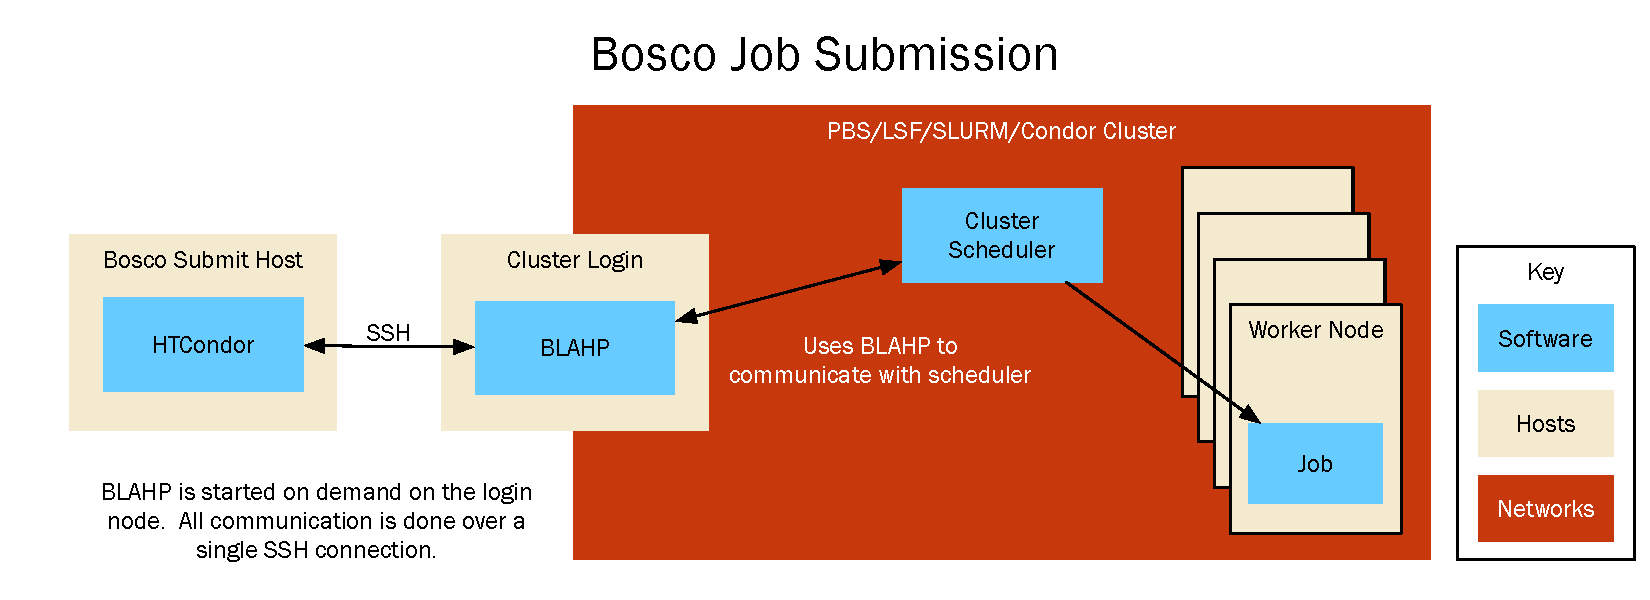
\includegraphics[width=\textwidth]{images/ArchitectureGraph1}
\caption{Bosco Architecture}
\label{fig:archgraph1}
\end{sidewaysfigure}

First, the Bosco submit node connects to the login node over an SSH connection and creates the forwarded SSH tunnel back to the submit node which is used for file transfer.  SSH was chosen as the protocol since it is used nearly universally for cluster access.  It creates the forwarded SSH tunnel in order to minimize the number of connections between the Bosco submit host and the login node.  By reusing the same SSH connection, we reduce the number of SSH logins to 1.  Further, the number of connections is not dependent on the number of jobs, as Bosco will reuse the same connection for all jobs submitted to a cluster.  Minimizing the number of connections to a login node is important since many login nodes include firewall rules to slow down brute force SSH logins that block frequent successive SSH connections.  The Bosco submit host does not require any open ports in a firewall, only outgoing connections to remote login node's SSH port.

%    Jobs are submitted to Bosco, which then submits over ssh to the remote cluster.  Input files are transferred over the SSH connection as well.  Bosco then monitors and reports the status of the job on the remote cluster as idle, running, or completed.  Once the job is completed, Bosco will transfer output files back to the submit host.


Next, Bosco checks for the necessary installed software on the login node, and starts the BLAHP \cite{blahp} daemon that will communicate with the scheduler on the login node.  The BLAHP daemon on the login node starts the file transfer daemon to connect back to the submit host through a forwarded SSH tunnel that Bosco created.  The transfer daemon creates and transfers the job sandbox to the login node.  The transfer to the login node is performed by HTCondor's fault tolerant file transfer mechanisms and are entirely encrypted over the SSH connection.  Authentication between the login node and the Bosco submit host is performed by a shared secret that was previously sent over the SSH connection to the BLAHP daemon.

After the files have been transferred, Bosco sends the job's submission ClassAd \cite{raman1998matchmaking} to the BLAHP daemon to translate to the local site's scheduler language.  The BLAHP supports PBS \cite{computing2013torque}, LSF \cite{computinglsf}, SGE \cite{gentzsch2001sun}, SLURM \cite{yoo2003slurm}, and HTCondor schedulers.  The BLAHP creates the submission file, and submits to the cluster's scheduler.  Bosco periodically polls the BLAHP over the SSH connection for the status of the job.  Once the job is detected to have been completed, the BLAHP starts HTCondor's transfer daemon to transfer the output sandbox back to the submitter machine.

Bosco has two modes of job submission:
\begin{enumerate}
	\item \textbf{Direct} -- A single job on the Bosco submit host corresponds to a single job on the remote cluster.  Each job is submitted individually to the remote cluster's scheduling system.  This method is the simplest to run, and imposes no special requirements on the submit machine.
	\item \textbf{Glidein} -- Bosco submits many pilot jobs to the remote cluster using the Direct method.  But, each of the pilots can service multiple user submitted jobs from the Bosco submit host.  This method minimizes the overhead on the remote cluster since Bosco is not submitting many jobs through the cluster scheduler.  The Glidein method requires that the Bosco submit host can be contacted from the remote cluster worker nodes. \label{sec:glidein}  The Glidein submission method is based off of previously written software such as the Campus Factory \cite{weitzel2011campus}.
\end{enumerate}

The two modes of job submission allow users to optimize for their environment.  If they are running many short identical jobs (which is frequent in High Throughput Computing), then the Glidein method is ideal for them.  If they are running fewer, longer, and possibly unique requirement jobs, then the direct submission method would work best.  Most users start with the direct method then graduate to glidein once they become accustomed to submitting batch jobs.

Bosco's fault tolerance is in it's handling of the remote cluster.  For example, if the user's computer loses connection with the remote cluster due to network issues, or even if the user suspends their laptop, Bosco will place the jobs on hold.  Although no new jobs will be submitted to the remote cluster, jobs that were already submitted will continue to run.  Further, when Bosco re-establishes a connection to the remote cluster, Bosco will check the status of already submitted, bring back any output data from any that have completed, and continue to submit jobs to the remote scheduler.

\subsection{Improving User Experience}

In order to improve the user experience, at each step of the job process, extra effort has been given to provide useful error messages in case of failures.  For example, HTCondor was modified to relay the standard error for any commands sent to the BLAHP daemon, as useful debugging information is available there.  

Also, an additional \emph{traceroute} was created to test each step of the job submission process, including:

\begin{enumerate}
\item SSH connection to the remote login host.  Tests network connection, login host availability, passwordless SSH setup.
\item Job submission to the Bosco submit host.  Tests Bosco daemon availability, Bosco submit host file system availability.
\item Job submission to the remote login host.  Tests the remote scheduler availability, remote cluster software setup, input file transfer, cluster file system availability.
\item Job completion and status update from login host.  Tests Bosco status check process, output file transfer.
\end{enumerate}

The \emph{traceroute} is very useful for debugging issues with a Bosco installation.  It is designed to test each step in the job execution life cycle and give meaningful error messages and possible solutions.

\section{Load Balanced Access to Computational Resources}

Bosco is used in conjunction with the Campus Factory \cite{website:campusfactory}, which is described in full in my Master's thesis \cite{weitzel2011campus}.  The Campus factory submits pilot jobs to remote clusters to create an overlay that provides a consistent interface to the resources.  The campus factory submits to multiple Bosco endpoints simultaneously, load balancing between them by keeping idle jobs (constant pressure) on all clusters.

Submission via the Bosco framework is done using the HTCondor submit syntax.  When an idle user job is detected by the Campus Factory, it begins to submit glideins to all Bosco endpoints simultaneously.  The Campus Factory maintains idle glideins on each of the endpoints until the user jobs have completed.  The jobs run on any resources that become available.


\section{BoscoR: Extending R from the desktop to the Grid}

As a case study of improving the user experience when using Bosco and distributed computing, we created BoscoR, an interface to Bosco from the R statistical programming language.  The following was published as:

\bibentry{weitzelboscor}

\subsection{Introduction}
Usage of the R language \cite{team2012r} by data miners has grown much faster than any other programming language \cite{rexer2013, KDnuggets2013}.  Data mining requires computational resources, sometimes more computational resources than can be provided by their desktop.  In a recent study \cite{rexer2013}, ``Available computing power'' was the second most common problem for big data analysis.  In addition, the respondents stated that distributed or parallel processing was the least common solution to their big data needs.  This could be attributed to the difficulty of processing data with the R language on distributed resources, a challenge we set out to solve with BoscoR.

A reason that distributed computing is not seen as a popular solution to big data processing is that scientists are more familiar processing on their desktop than in a cluster environment.  R is typically used by people that have not used distributed computing before and do most of their analysis on their local systems with IDEs such as RStudio \cite{racine2012rstudio}.  Users are unaccustomed to the traditional distributed computing model of batch processing in which there is no interactive access to the running processes.

Though researchers may not have experience with distributed computing, most have computational resources available to them, either locally provided by their institution or university, or through national cyberinfrastructure such as the OSG \cite{pordes2007open} or XSEDE \cite{xsede}.



In this section, we will describe GridR \cite{wegener2007gridr}, a R library used to interact with the Bosco framework.  In section \ref{sec:boscorimplementation}, we describe how we combined these two components to create a fault tolerant framework that provides a positive user experience.  Next, in Section \ref{sec:boscorresults}, we discuss preferred submission methods based on the length of the R function, and show some results from numerous test runs against a production cluster.  Finally, we offer some conclusions and future work.

\subsection{Background}
BoscoR is primarily made up of two components, Bosco and GridR.  Bosco provides an simple to setup interface to the remote batch system, and provides fault tolerance for job submission and file transfers.  GridR provides a user interface to create and initiate remote processing.


\subsection{GridR}
% Overview of parallel libraries
Many parallel libraries are available for R.  Most focus on managing the R processing on a single server such as the \texttt{parallel} package \cite{rparallelpackage}.  The \texttt{parallel} package comes bundled with R and provides for single machine parallelism.  Parallelism is done by using variations of the R function \texttt{lapply}.  A simplified definition of \texttt{lapply} is shown in Figure \ref{lst:lapply}.  \texttt{lapply} is the basis for nearly all parallel libraries in R.  

\begin{figure}[ht!]
\begin{framed}
\texttt{lapply}(\textbf{X}, \textbf{FUN}, \textbf{\ldots}):
\begin{description}
\item[\textbf{X}] a vector (atomic or list) or an expression object.
\item[\textbf{FUN}] the function to be applied to each element of X
\item[\textbf{\ldots}] optional arguments to FUN.
\item[Returns] list of the same length as X, each element of which is the result of applying FUN to the corresponding element of X.
\end{description}
\end{framed}

\centering
\captionsetup{justification=centering}
\caption{Funciton definition of \texttt{lapply}}
\label{lst:lapply}
\end{figure}

The \texttt{lapply} function is ideally suited for high throughput computing.  There is no communication between executions of the function on the array.  The input vector can be easily partitioned in order to split the execution across multiple resources.  It is because of these reasons that most parallel applications use the \texttt{lapply} model to provide parallelism.  Examples are the parallel package which defines the functions \texttt{mcapply} (multi-core apply) and \texttt{parapply} (parallel apply). In the \texttt{parallel} package, calling \texttt{mcapply} causes R to fork a process that will execute the function \textbf{FUN} on each element in the input vector.  A similar process happens when calling \texttt{parapply}. 

Another built-in parallelization package is Simple Network of Workstations (snow) \cite{rlangsnow}.  Snow allows for multiple computers to organize and execute parallel processing of data.  The computers communicate over regular network sockets or using MPI \cite{gropp1999using}.  This allows for multiple computers inside the same cluster to process data.  Snow also has built-in \texttt{lapply} style functionality.

GridR also follows this \texttt{lapply} model for parallelization.  It uses a function called \texttt{grid.apply}, which will apply a function to every element of an input vector, similar to \texttt{lapply}.  Instead of forking a process like \texttt{mcapply}, it compiles the input data and function, and submits the execution to a grid endpoint.

GridR was originally written for use with data analysis in ACGT clinico-genomics trials \cite{wegener2007gridr}.  It was written with the capability to submit with a limited set of grid protocols, some of which are no longer supported.  Further, GridR made assumptions of the remote resources.  These assumptions were:

\begin{itemize}
\item R is installed on all of the worker nodes.
\item The R binaries are in the same location on all of the remote resources.
\item The GridR package is installed on all of the remote resources.
\end{itemize}

All of these assumptions cannot be met on modern grid resources.  Applications cannot assume that a (non-standard) processing tool, such as R, is installed on every computer or   that it is installed at exactly the same location on all clusters in the grid.  Modifications were made to GridR to erase these assumptions, as well as to adapt it to submit to Bosco.

\subsection{Implementation}
\label{sec:boscorimplementation}

% \begin{itemize}
% \item Combining Bosco with GridR improves usability dramatically for R users.
% \item Modify GridR in order to submit to local bosco
% \item Improve scalability and fault tolerance of GridR
% \item Downloads appropriate version of R from a central repository.  Caches the R installation if available (both at the file system level, and the R level).
% \end{itemize}

Bosco is designed to run on resources that are not controlled by the submitting user.  Further, it is designed to run on resources without any conditions as to what is installed.  In order to operate under these assumptions, Bosco must bootstrap itself by bringing in all the libraries and dependencies required to operate.  Therefore, BoscoR must run under these same assumptions.

GridR was modified to submit to Bosco.  The input generation of GridR is shown in Figure \ref{fig:gridrinput}.  When a user or script calls \texttt{grid.apply}, GridR compiles the input function and input data into a R data file, which can be read later by another R process.  GridR handles function dependencies by using R's dependency detection and compiles any functions that may be required into the input.  

\begin{figure}[ht]
\centering
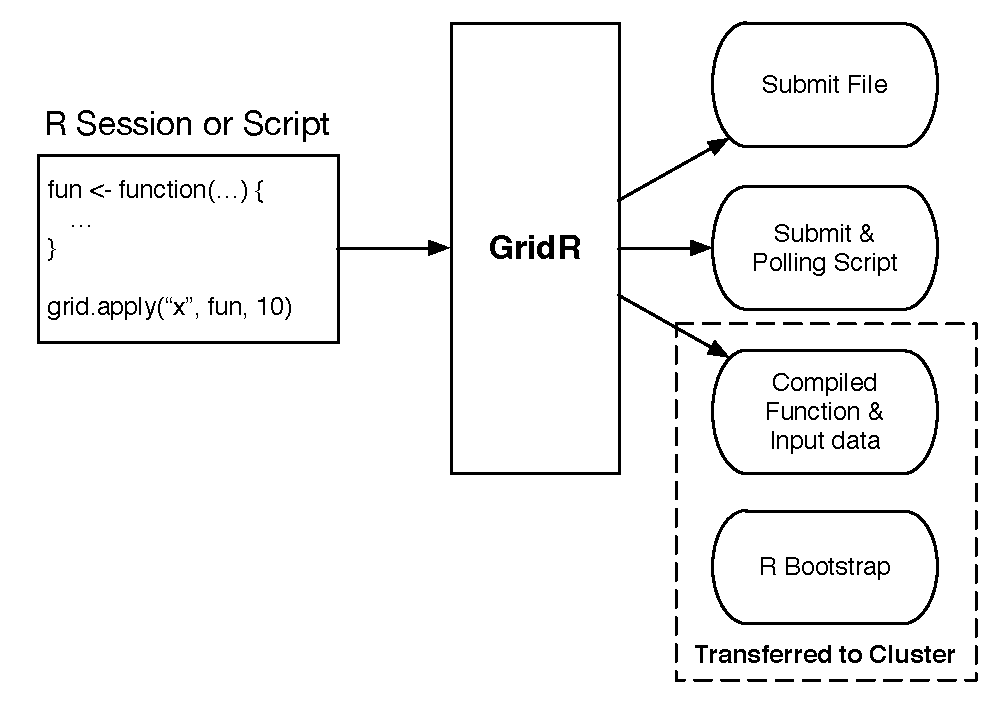
\includegraphics[width=\textwidth]{BoscoRImages/InputDiagram.pdf}
\caption{GridR Input Generation}
\label{fig:gridrinput}
\end{figure}

GridR was modified to first create a submit file which will be submitted to the local system where Bosco is installed.  The submit file explicitly lists the input files and the expected output file, all of which will be transferred by Bosco.  The input files, as shown in Figure \ref{fig:gridrinput}, are the compiled function and input data and a bootstrap executable.  The output file contains the return value from the executed function.

The submit and polling script is executed by GridR after forking a new R process.  This is a light weight process that submits the Bosco submission script and watches for any errors.  If the input function is executed many times by many separate jobs, the polling script will aggregate the results as they are returned to the submit node into a vector that will be returned to the user.  

\subsection{Bootstrap}
\label{sec:boscorbootstrap}

Since Bosco cannot make assumptions as to what is installed on the remote cluster, neither can BoscoR.  Therefore, GridR was modified to detect, and if necessary install, R on the remote system.  This was performed by a bootstrap process.

In the GridR generated submit file, the listed executable to run on the remote system is not R, but the bootstrap executable.  The bootstrap executable detects if R is installed on the remote system.  If it is installed, it simply executes the user defined function against the input data.  If R is not installed, the bootstrap downloads the appropriate version of R for the remote operating system.  The supported platforms are identical to Bosco's, CentOS 5/6 and Debian 6/7.  R is downloaded from a central server operated by the OSG's Grid Operations Center \cite{osgoperations}.  

The bootstrap executable installs R in a shared directory.  By utilizing a shared directory, subsequent GridR jobs may use the same R installation.  Several bootstrap jobs could start at once on a remote cluster, so a simple transactional file locking mechanism was devised so only a single bootstrap executable on a cluster will download and install for the entire cluster if a shared file system is available.  If a shared filesystem is not available for installation, R is installed in a temporary directory that is removed upon job completion.

\subsection{Running on the Open Science Grid}

Submitting to the Open Science Grid (OSG) is done by direct submission.  The OSG hosts access nodes which can be used to submit to resources on the grid.

Most OSG sites do not have shared directories for grid users.  Therefore, the bootstrap script must install R on every node in a temporary directory.  In order to optimize the R installation, the bootstrap script utilizes the HTTP forward proxy infrastructure \cite{garzoglio2012supporting} available on the OSG to minimize requests to the central hosting server.


\subsection{Results}
\label{sec:boscorresults}

The results section is broken into two categories, results from user feedback and results from experimental runs on a production cluster as well as the OSG.

A primary goal with BoscoR was to improve the user experience of using R on distributed resources. After acquiring a few users, we received feedback on how BoscoR could be improved.  The improvements to GridR and the integration with Bosco made working with campus or institutional resources much better.  In this section we will describe the improvements.

\subsubsection{User Provided Packages}

Many users require additional packages to be installed before their function can execute.  It was assumed that most of these packages would be in the major R package repositories, such as the Comprehensive R Archive Network (CRAN) \cite{cran}.  If the package is in CRAN, the user provided function can install the package.  After receiving user feedback, it was found that not all desired packages are available in CRAN.  A modification to both the submit file and the bootstrap executable was designed to install such packages.

In order to install a user provided package, it first needs to be transferred to the remote cluster.  This is done by including the package in the list of input files to be transferred by Bosco for each job.  Additionally, the packages should be installed before the user function is executed on the remote resources.  This required modification to the bootstrap executable in order to install the packages after installing R, but before executing the user's function on the input data.

\subsubsection{Quick Jobs}
Since the GridR interface only provides for a single function to execute against the input data, it was assumed that the function would be a time consuming data processing function that may call many other functions.  Therefore, the overhead Bosco introduces would not significantly effect the performance of the executions.  After receiving feedback from users, it was determined that the more common use case is to use smaller functions that could execute in seconds or minutes.  In order to accommodate shorter jobs, a modification to the GridR generated submit script was required.

In this case, we modified the submit file so that Bosco would use the Glidein method of job submission.  Using the Glidein job submission method, the shorter jobs can be executed much more quickly, one after another, reusing the same resources.  Additionally, this saves the remote cluster scheduler from scheduling many small jobs which can cause issues in many HPC schedulers.


\subsection{Performance Results}

\subsubsection{Experimental setup}  

In order to test BoscoR, we have to simulate a R workload.  We simulate a workload with varying lengths of the executed functions.  This simulates a variety of workloads that we have seen from users.  As noted before, we assumed that the functions would be long running data processing.  But, we learned that users were instead submitting short functions to be executed quickly.  We varied the length of function from 1 second to 30 minutes.  To verify our solution to quick jobs, we tested different job lengths using both the Direct and Glidein submission method.

To execute the test jobs, we used the production cluster \textit{Tusker} at the University of Nebraska -- Lincoln Holland Computing Center.  This cluster is composed of 106 nodes, each with 64 cores, for a total of 6784 cores.  The cluster has numerous users that are submitting to the central SLURM \cite{yoo2003slurm} scheduler.  The cluster traditionally runs at $>$90\% utilization, with dozens of users jobs fair sharing the resources.  The SLURM scheduler is a HPC orientated scheduler that matches submitted jobs to resources.  Fair share scheduling is used on Tusker.  Each group has equal priority with all others, therefore allowing the maximum number of users to run on the resources.

The Tusker cluster was chosen since access was easy for the authors of this paper.  Further, it is utilized enough that the jobs would be competing against other user's jobs for available resources, and therefore not all submitted GridR functions would be able to execute simultaneously.  We believe this best represents most clusters, which are typically highly utilized by many researchers.  It is plausible that a cluster could be so utilized that no user jobs could be executed, while the other extreme could also be true, that enough resources are available for all submitted jobs to be executed immediately.  We found that Tusker utilization is somewhere between these two extremes.  It is capable of running many, but not all, jobs submitted to it immediately.  The rest will execute as resources become available.

For our testing, we submitted 1000 GridR jobs per test run. 1000 jobs was chosen as a reasonable representation of workflows we have seen when helping users of GridR.  They typically submit many jobs, sometimes reaching into the thousands.  Our goal was to submit more jobs than could be run instantly by the remote cluster, but no so many that gathering repeated testing data would be impossibly time consuming.

\subsubsection{Direct submission}
Direct submission is defined as submission using Bosco's direct submission method.  In GridR, the library is initialized with the argument \texttt{service="bosco.direct"}.  When this setting is used, GridR generates submission scripts that use Bosco's default routing mechanism to submit to a single cluster.  The GridR functions are submitted as jobs directly to Tusker's SLURM scheduler.

\begin{figure}[ht!]
\centering
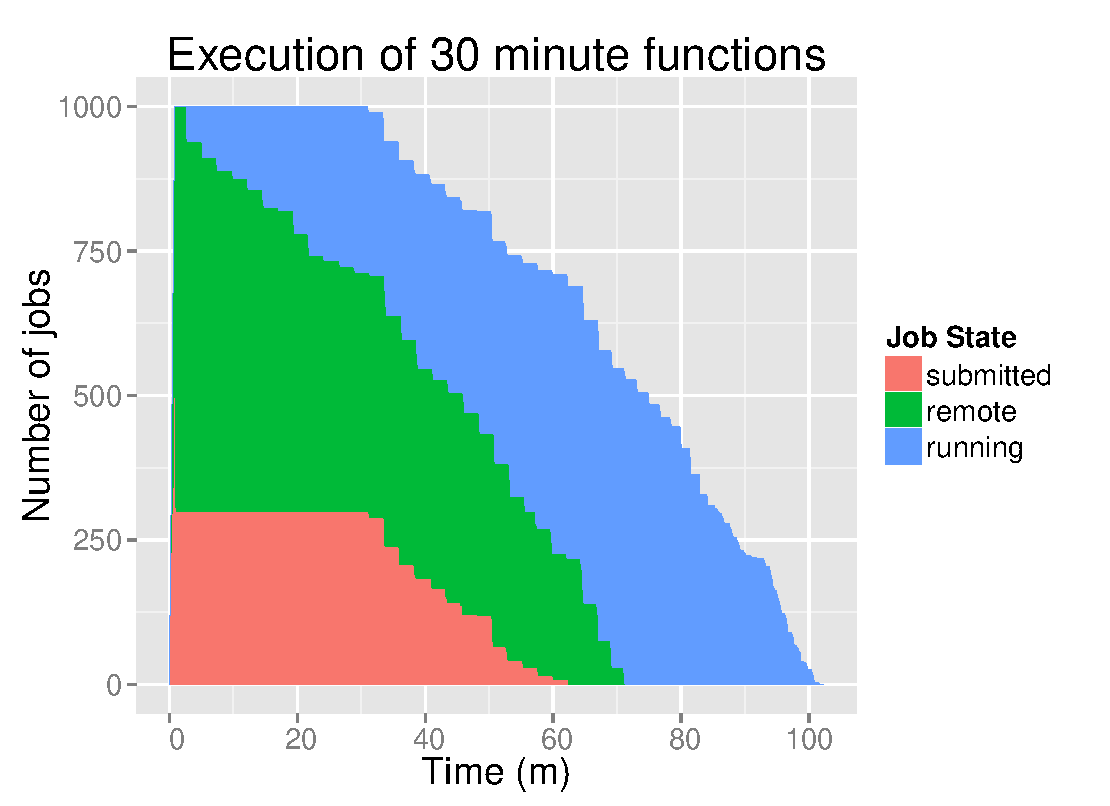
\includegraphics[width=\textwidth]{BoscoRImages/30minplot.pdf}

\caption{Direct submission}
\label{fig:directsubmit}
\end{figure}

A timeline of the GridR submissions to Bosco is shown in Figure \ref{fig:directsubmit}.  The submitted jobs are jobs which are submitted locally, but not yet submitted to the remote scheduler.  Remote represents the jobs which are submitted to the remote SLURM scheduler.  The submission to the remote scheduler is very rapid.  Bosco is able to submit 700 jobs, the limit in this implementation to submit at a single time, within a minute.  SLURM is able to rapidly begin executing many, but not all, of the submitted jobs.  Bosco maintains constant pressure in the form of idle jobs in case resources become available on the cluster.  You will notice the straight line in the number of submitted jobs which dips after 30 minutes.  At 30 minutes the first jobs begin to complete and Bosco begins to submit more jobs to the cluster, attempting to always keep the maximum of 700 jobs either idle or running on the remote cluster.  In this workflow, all 1000 30 minute jobs finish in just over 100 minutes.

The Open Science Grid runs use the direct submission method as well.  But, since the OSG access nodes run HTCondor, the jobs are capable of starting much quicker after being submitted to the remote resource.  In this way, the OSG provides the best of both the direct and glidein approaches.  It is simple to setup like any direct submission method.  And as with the glidein submission method, the jobs start quickly on the remote resource.

The OSG direct submission presents different failure modes than a traditional HPC cluster.  For example, in one of our experimental runs with 1 second jobs, a single job took over 30 minutes to complete.  The issue with this particular job was that the job was matched to a single node that was misconfigured.  In this case, the job eventually finished after being matched to a different node.  The OSG may not be an ideal solution for short executions of GridR functions.

\subsubsection{Glidein}
Glidein submissions use a pilot that is submitted directly to the SLURM scheduler.  Once the pilot starts, it calls back to the submission node to request work.  This method allows multiple jobs to run within the same SLURM job, independent of the cluster's scheduler.  

\begin{figure}[ht!]
\centering
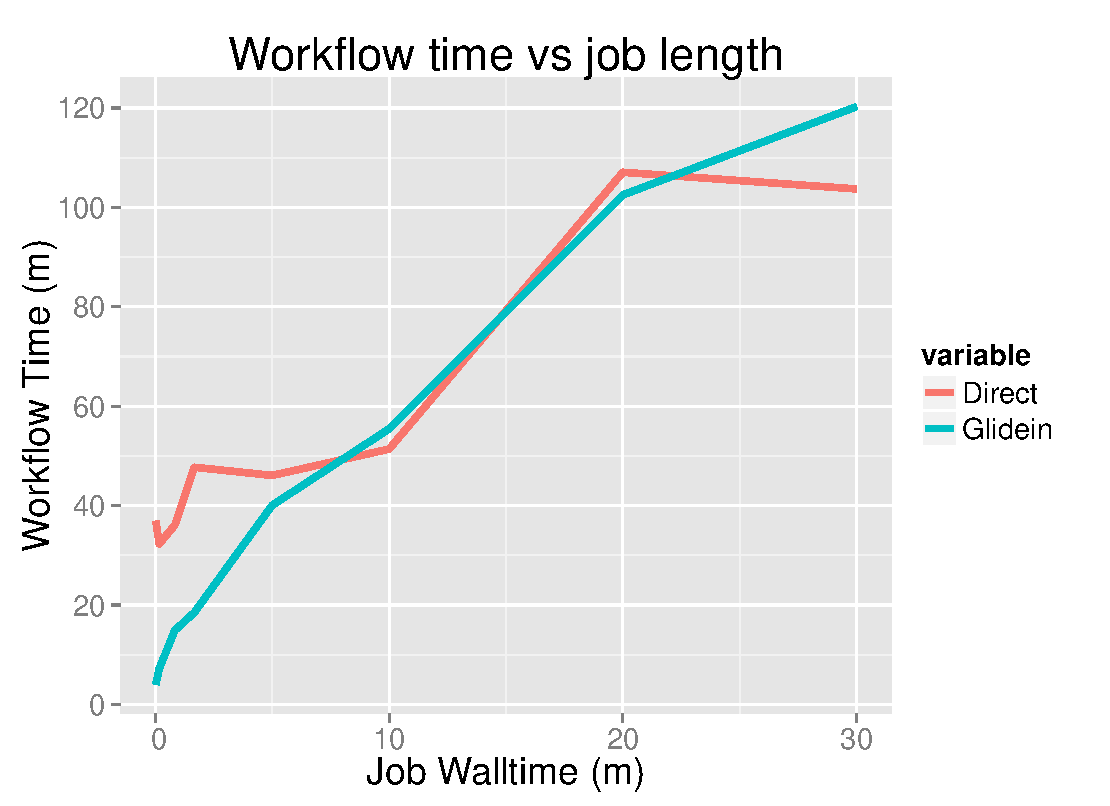
\includegraphics[width=\textwidth]{BoscoRImages/ComparisonPlot.pdf}
\caption{Comparison of submission methods}
\label{fig:comparesubmit}
\end{figure}

Comparing the Direct submission to the glidein submission is shown in Figure \ref{fig:comparesubmit}  As you can see, for longer jobs, direct and glidein submission methods have approximately similar workflow runtimes.  But, for short jobs, glidein has significantly shorter workflow runtimes.  This can be attributed to the advantages of using a high throughput scheduler over a high performance scheduler.

Bosco is built on top of HTCondor.  HTCondor is a very efficient high throughput scheduler that can quickly start the execution of jobs upon available resources.  Since many R workflows are designed to run a short function upon a large amount of data, HTCondor is a good fit.  By submitting HTCondor pilots to the remote scheduler, Bosco is able to utilize its strength of running many small jobs quickly, resulting in a shorter workflow completion time for shorter jobs.

\begin{figure}[ht!]
\centering
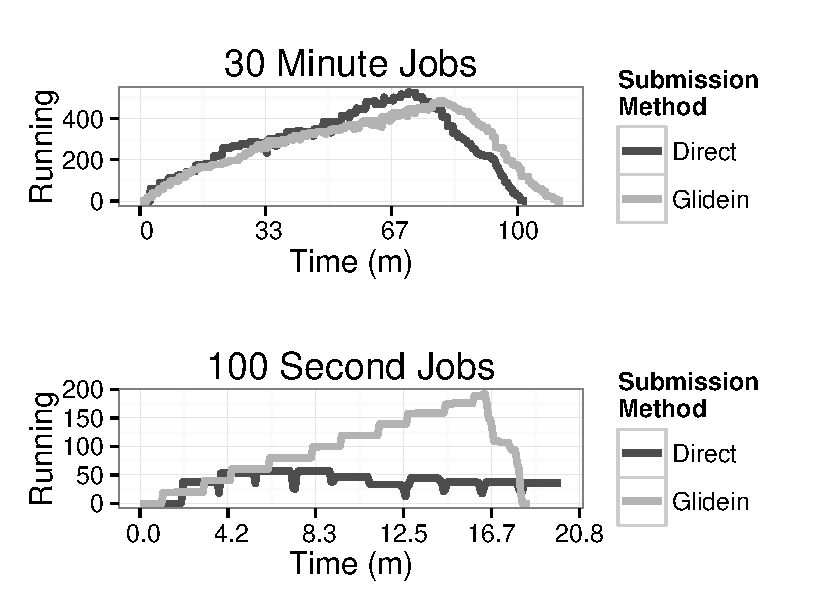
\includegraphics[width=\textwidth]{BoscoRImages/NumberRunning.pdf}

\caption{Number of simultaneously running jobs}
\label{fig:runningjobs}
\end{figure}

Figure \ref{fig:runningjobs} illustrates how the glidein submission method is superior to the direct submission method for short jobs, and why both methods are roughly equivalent for longer jobs.  For longer jobs, you can see that both glidein and direct submission methods start jobs at nearly equal rates.  The variation is relatively small, and could be explained by variations in the available resources at the time of running the experiments. 

For the shorter 100 second jobs the start rate begins nearly the same, but then Bosco and SLURM are unable to sustain the job start rate.  Since the jobs only run for 100 seconds the overhead from Bosco submission and SLURM starting the jobs becomes a bottleneck.  Bosco is only able to sustain roughly 50 jobs running on the cluster.  On the other hand, the Glidein submission method continues to grow in the number of jobs running.  This is due to eliminating the Bosco submission overhead, as well as the SLURM scheduling overhead.  Instead, the Glidein method is utilizing the much more efficient HTCondor scheduler, which is able to start jobs much faster than the SLURM scheduler.  We can conclude that the glidein submission method results in a shorter total workflow execution time for shorter R functions.


\subsection{Conclusion}

BoscoR is a framework to execute R functions on distributed resources.  It is a simple method for users to distribute processing to remote resources.  BoscoR incorporated user feedback in order to improve the framework.

As with any complicated system, many parameters can be varied in order to obtain different results.  For example:
\begin{itemize}
\item Resource contention may be high which could cause the cluster not to start any GridR jobs.
\item Resource contention may be low, which would cause SLURM to start all submitted jobs immediately.
\item The number of glideins submitted in a batch could be varied in order to optimize the start rate for a particular cluster.  Any lower and it would slow job starts, increasing the workflow run time for both short and long jobs.  Any higher, and it could overwhelm the remote scheduler.
\end{itemize}

We chose reasonable values for these parameters that an end user may use.  In the future we will tune these parameters automatically using the feedback provided by Bosco.  Although Bosco and the bootstrap process significantly improved the fault tolerance of GridR, further fault tolerance testing and development is needed to provide a positive user experience when running on national infrastructure such as the OSG.

During follow up interviews with users after using BoscoR, we received many positive reviews of the framework.  Improving the user experience of using R on distributed resources was a primary goal of BoscoR.  One example of a positive review was from a Micro-Biology researcher from the University of Wisconsin:
\begin{quote}
I have a huge set of data, which I have to split into pieces to be handled by each node.  This is something I can do with the "grid.apply" function. This reduces the submit time from several hours, to several seconds... it is a  phenomenal improvement. This will greatly increase my use of grid computing, as right now, I only use grid computing when I have no other choice.
\end{quote}

The experimental testing we ran showed that glidein submission method is significantly better at running short R functions than the direct submission method.  At longer job runtimes, the difference between direct and glidein submission to remote resources is negligible.






\section{Conclusion}

Bosco and the Campus Factory combine to make an easy to use framework that can distribute jobs to many computational clusters on a campus.  Users are able to effectively distribute their processing to multiple clusters using this framework.  In this section, I showed that Bosco transparently and effectively distributes computational jobs across multiple clusters on a campus, while maintaining simple usage for users.

Bosco's usage has increased since I originally published the Bosco paper.  For example, it is heavily used by the University of Chicago in order to submit OSG processing to opportunistic resources around the country.  They find Bosco useful since it does not require the installation of any software on the remote cluster.

Additionally, the CMS experiment has used Bosco to access opportunistic resources around the world, and has published many papers on the subject \cite{hufnagelcmsopportunistic, piperovoperationalchep15, wagner2013using, kreuzer2014opportunistic}.

If the user's workflow requires significant data, it may be inefficient to use Bosco's transfer mechanisms which are bottlenecked by the transfer speed of the Bosco submit host.  It is expected that large datasets will not be an efficient use of Bosco.  Therefore, we will introduce a framework to efficiently transfer data in Chapter \ref{chapter:campusdatadistribution} that will complement Bosco's overlay network.



